\documentclass[12pt,a4paper]{article}
\usepackage[margin=2.0cm]{geometry}
\usepackage[T1]{fontenc}
\usepackage{lmodern}
\usepackage{enumitem}
\usepackage{xcolor}
\usepackage{booktabs}
\usepackage{tabularx}
\usepackage{array}
\usepackage{tikz}
\usetikzlibrary{arrows.meta,positioning,fit,backgrounds}
\usepackage{caption}
\usepackage[hidelinks]{hyperref}
\usepackage{xurl}
\usepackage{titlesec}

\definecolor{head}{RGB}{25,60,120}
\titleformat{\section}{\Large\bfseries\color{head}}{\thesection.}{0.6em}{}
\titleformat{\subsection}{\large\bfseries\color{head}}{\thesubsection}{0.6em}{}
\setlist{itemsep=3pt,topsep=4pt,leftmargin=1.5em}
\setlength{\parindent}{0pt}
\setlength{\parskip}{6pt}
\linespread{1.05}
\renewcommand{\arraystretch}{1.25}
\newcolumntype{L}{>{\raggedright\arraybackslash}X}

\tikzset{
  box/.style={draw, rounded corners=3pt, align=center, minimum height=1.0cm, text width=2.6cm, font=\small, fill=#1},
  box/.default={white},
  arr/.style={-{Stealth[length=2.5mm]}, thick},
  layer/.style={draw, dashed, rounded corners=6pt, inner sep=8pt}
}

\begin{document}

%================ TITLE PAGE ================
\begin{titlepage}
\centering
\vspace*{2cm}
{\large IT457 -- Cloud Computing\par}
\vspace{0.4cm}
{\large Case Study Project\par}
\vspace{2cm}
{\Huge\bfseries\color{head} GE Predix\par}
\vspace{0.4cm}
{\LARGE Industrial IoT Cloud Platform and\\[4pt] GE's Migration to the Cloud\par}
\vspace{1.5cm}
{\Large Week 2 Report: Detailed Case Analysis,\\[4pt] Exercise Plan and Team Roles\par}
\vspace{2.5cm}
{\large\bfseries Group 27\par}
\vspace{0.3cm}
{\large Theme: Migration \& Transformation\par}
\vspace{1cm}
\begin{tabular}{ll}
\toprule
\textbf{Student ID} & \textbf{Name} \\
\midrule
202303009 & Nidhi Dodiya \\
202303046 & Param Savjani \\
202301436 & Vraj Makwana \\
\bottomrule
\end{tabular}
\vfill
{\large \today\par}
\end{titlepage}

\setcounter{tocdepth}{1}
\tableofcontents
\newpage

%================ 1 INTRODUCTION ================
\section{Introduction}
Most cloud success stories come from internet companies such as Netflix or Airbnb.
General Electric (GE) is different: it is a 130-year-old industrial company that builds jet engines,
gas turbines, locomotives and medical equipment. Around 2013 GE decided that software and data would be as
important to its future as hardware, and set out to become a ``digital industrial'' company.

This decision produced two connected cloud stories:
\begin{enumerate}
  \item \textbf{Predix}, a cloud platform built by GE for the \emph{Industrial Internet of Things (IIoT)}. It was
        designed to collect data from industrial machines, analyse it, and predict failures before they happen [1,2].
  \item \textbf{GE's own IT migration}, in which GE moved thousands of internal applications out of its private
        data centers and onto Amazon Web Services (AWS) [4,5].
\end{enumerate}

This report studies both stories in detail. It explains the problem GE was trying to solve, the architecture of the
solution, the cost and business outcome, and the lessons for cloud computing. It then presents our plan for a
hands-on exercise that reproduces the core idea of the case on a small scale: a sensor-data application that is
migrated from a local Docker setup to a cloud VM, and then refactored to use managed cloud services.

%================ 2 BACKGROUND ================
\section{Background}
\subsection{GE and the Industrial Internet}
GE's machines operate in some of the most critical environments in the world: power plants, aircraft, railways and
hospitals. Each machine is fitted with many sensors. A single gas turbine or jet engine can produce large volumes of
data every hour of operation. Historically, this data was used only locally, for real-time control, and then mostly
discarded.

GE coined the term \emph{Industrial Internet} for the idea of connecting these machines to the network, collecting
their data centrally, and applying analytics to improve efficiency. Even small improvements matter at this scale:
a 1\% fuel saving across an airline fleet or a power grid is worth a very large amount of money.

\subsection{Timeline}
\begin{center}
\begin{tabularx}{\linewidth}{@{}p{2.2cm}L@{}}
\toprule
\textbf{Year} & \textbf{Event} \\
\midrule
2013 & GE launches Predix as its software platform for the Industrial Internet of Things [3,9]. \\
2013 & GE invests \$105 million in Pivotal, the company that led the Cloud Foundry project [3]. \\
2015 & GE Digital is formed. In August, GE announces \textbf{Predix Cloud}, a PaaS for industrial data [1]. \\
2015 & At AWS re:Invent, GE's CIO presents the plan to move 9,000 workloads to AWS and shrink from 34 data centers to 4 [4]. \\
2016 & Predix Cloud becomes commercially available to external customers [3]. \\
2017 & GE names AWS its \emph{preferred cloud provider}; over 2,000 applications already migrated [5]. \\
2017 & Reports of technical problems; Predix takes a ``time out'' from the market [7]. \\
2018 & New leadership refocuses GE Digital on Power, Aviation and Healthcare and cuts costs [8]. \\
Dec 2018 & GE announces plans for a separate industrial IoT software company with \$1.2B revenue [9]. \\
Oct 2019 & GE decides to keep GE Digital inside the company, with a narrower vertical focus [9]. \\
\bottomrule
\end{tabularx}
\end{center}

%================ 3 PROBLEM ================
\section{Problem Statement}
GE faced two separate but related problems: one on the product side and one on the internal IT side.

\subsection{Problem 1: Unused industrial data}
\begin{itemize}
  \item \textbf{Volume and velocity:} industrial machines generate continuous, high-frequency time-series data. Traditional
        enterprise databases and on-premises servers were not designed for this load.
  \item \textbf{Unplanned downtime is expensive:} when a turbine or engine fails without warning, the cost includes
        repairs, lost production and safety risk. Customers wanted \emph{predictive maintenance}, meaning that
        the machine's data should warn them before a failure happens.
  \item \textbf{Remote and unreliable connectivity:} machines are often located at remote sites such as oil rigs, wind farms or
        aircraft, where network connections are slow or intermittent.
  \item \textbf{Security and reliability:} the data comes from critical infrastructure, so the platform must be highly
        secure and always available.
  \item \textbf{Generic clouds lacked industrial features:} in 2015, general public clouds did not offer ready-made
        services for industrial protocols, asset models or physics-based analytics.
\end{itemize}

\subsection{Problem 2: Expensive, fragmented internal IT}
\begin{itemize}
  \item GE had grown through decades of acquisitions, leaving it with a very large and fragmented IT estate: around
        \textbf{9,000 workloads spread across 34 data centers} in 2015 [4].
  \item Running so many data centers meant high fixed costs for hardware, power, cooling, staff and maintenance.
  \item Provisioning new servers was slow, which slowed down development teams.
  \item Many duplicated systems existed across business units, making the estate hard to manage and secure.
\end{itemize}

\subsection{Why the cloud?}
Both problems point to the same core benefits of cloud computing: \emph{elastic} storage and compute that can grow with
data volume, \emph{pay-as-you-go} pricing instead of large up-front investment, \emph{managed services} that remove
operational work, and \emph{global reach} for customers and machines located around the world.

%================ 4 SOLUTION ================
\section{Solution and Architecture}
\subsection{Predix platform overview}
Predix was designed as a \textbf{Platform-as-a-Service (PaaS)} for industrial applications. Its architecture has three
main tiers: the \emph{edge}, the \emph{cloud platform}, and the \emph{applications} built on top [1,6].

\begin{figure}[h]
\centering
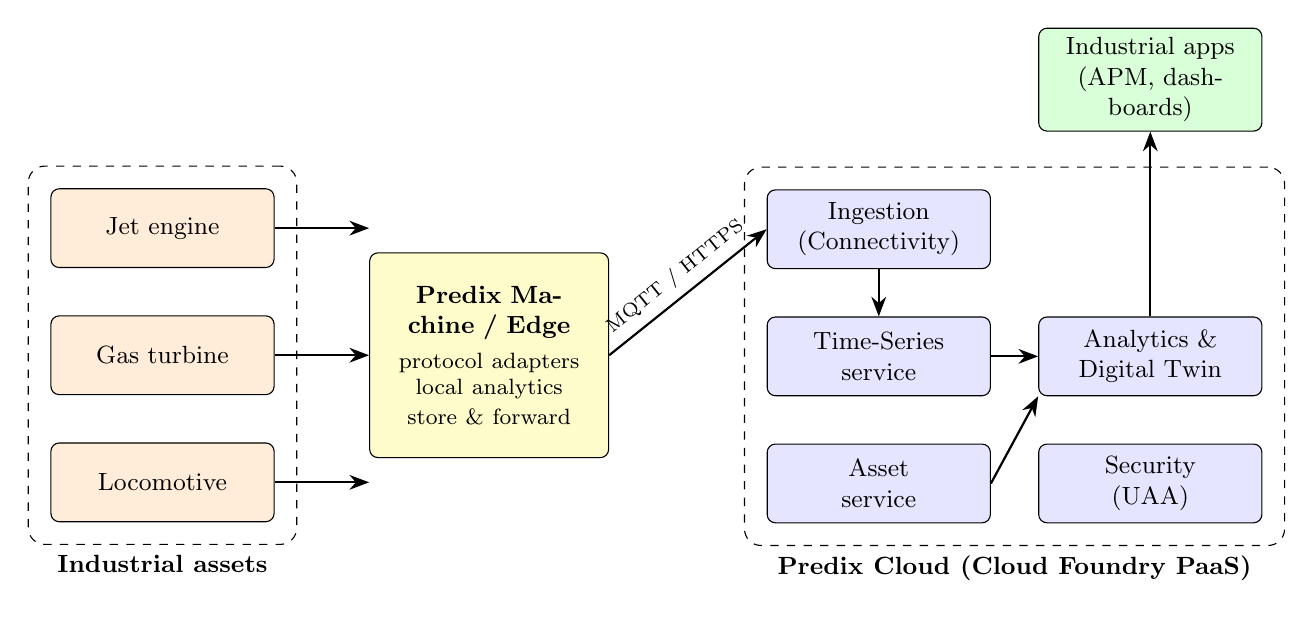
\begin{tikzpicture}[node distance=0.6cm and 0.6cm]
  % Assets
  \node[box=orange!15] (a1) {Jet engine};
  \node[box=orange!15, below=of a1] (a2) {Gas turbine};
  \node[box=orange!15, below=of a2] (a3) {Locomotive};
  % Edge
  \node[box=yellow!20, right=1.2cm of a2, text width=2.8cm, minimum height=2.6cm] (edge)
       {\textbf{Predix Machine / Edge}\\[3pt]\footnotesize protocol adapters\\ local analytics\\ store \& forward};
  % Cloud
  \node[box=blue!10, right=2.0cm of edge, yshift=1.6cm] (ingest) {Ingestion\\(Connectivity)};
  \node[box=blue!10, below=of ingest] (ts) {Time-Series\\service};
  \node[box=blue!10, below=of ts] (asset) {Asset\\service};
  \node[box=blue!10, right=0.6cm of ts] (analytics) {Analytics \&\\Digital Twin};
  \node[box=blue!10, below=of analytics] (sec) {Security\\(UAA)};
  % Apps
  \node[box=green!15] (apps) at ([yshift=1.9cm]analytics |- ingest) {Industrial apps\\(APM, dashboards)};
  % arrows
  \draw[arr] (a1.east) -- (edge.west |- a1.east);
  \draw[arr] (a2.east) -- (edge.west);
  \draw[arr] (a3.east) -- (edge.west |- a3.east);
  \draw[arr] (edge.east) -- node[midway, above, sloped, font=\scriptsize]{MQTT / HTTPS} (ingest.west);
  \draw[arr] (ingest) -- (ts);
  \draw[arr] (ts) -- (analytics);
  \draw[arr] (asset.east) -- (analytics.south west);
  \draw[arr] (analytics) -- (apps);
  % layers
  \begin{scope}[on background layer]
    \node[layer, fit=(ingest)(asset)(analytics)(sec), label={[font=\small\bfseries]below:Predix Cloud (Cloud Foundry PaaS)}] {};
    \node[layer, fit=(a1)(a3), label={[font=\small\bfseries]below:Industrial assets}] {};
  \end{scope}
\end{tikzpicture}
\caption{Simplified Predix architecture: assets $\rightarrow$ edge $\rightarrow$ cloud services $\rightarrow$ applications.}
\end{figure}

\subsection{Edge tier: Predix Machine}
Predix Machine (later Predix Edge) is software that runs on a gateway next to the machine, or on the machine's controller.
Its responsibilities are [6]:
\begin{itemize}
  \item \textbf{Connectivity:} read data using industrial protocols such as OPC-UA and Modbus, and send it to the cloud
        using standard protocols such as MQTT, HTTPS and WebSocket.
  \item \textbf{Edge analytics:} run simple analytics locally, so that urgent decisions do not wait for the cloud.
  \item \textbf{Store and forward:} buffer data when the network is down and upload it when connectivity returns.
  \item \textbf{Fleet management:} Predix EdgeManager lets operators monitor and update thousands of edge devices centrally.
\end{itemize}
This edge-plus-cloud pattern is now standard in IoT and is offered by services such as AWS IoT Greengrass and Azure IoT Edge.

\subsection{Cloud tier: Predix Cloud on Cloud Foundry}
Predix Cloud was built on \textbf{Cloud Foundry}, an open-source PaaS, using Pivotal's distribution [1,2]. Developers
push their code, and the platform handles building, deploying, scaling and running it as \emph{microservices}. The
platform offered a catalogue of reusable services [6]:
\begin{itemize}
  \item \textbf{Time-Series service:} ingests and stores large volumes of timestamped sensor readings and supports fast queries.
  \item \textbf{Asset service:} models the physical hierarchy of equipment (system $\rightarrow$ subsystem $\rightarrow$ component $\rightarrow$ sensor) and tracks configuration changes.
  \item \textbf{Analytics runtime:} runs analytic models (rules, physics models, machine learning) on incoming data.
  \item \textbf{Security (UAA):} user account and authentication service for identity and access control.
  \item \textbf{UI components:} reusable widgets for building dashboards.
\end{itemize}

\subsection{Digital Twin}
A central concept in Predix is the \textbf{digital twin}: a software model of a specific physical machine. It
combines live sensor data, the machine's configuration and history, and physics or machine-learning models [6]. The
twin describes the asset's \emph{past} (its full history), its \emph{present} (current key performance indicators) and
its \emph{future} (predicted wear and failure). For example, a twin of a jet engine can estimate when a part will need
maintenance based on the actual conditions it has flown in, rather than on a fixed schedule.

\subsection{Deployment model}
In the beginning, GE ran production Predix workloads in its own data centers, while AWS was used for development and
testing [3]. GE later made Predix available on public clouds, including Microsoft Azure and AWS, so that customers
could choose where to run it. This is an example of a \emph{hybrid} and eventually \emph{multi-cloud} strategy.

\subsection{GE's internal IT migration to AWS}
In parallel with Predix, GE's corporate IT adopted a \textbf{cloud-first} strategy. The goal announced in 2015 was to
move most of its 9,000 workloads to AWS and reduce its data centers from 34 to 4, keeping only the most sensitive
systems on-premises [4]. By October 2017 GE had migrated more than 2,000 applications, and it named AWS its preferred
cloud provider. Several migrated applications use AWS analytics and machine-learning services [5].

Large migrations like this generally use a mix of strategies:
\begin{center}
\begin{tabularx}{\linewidth}{@{}p{3.4cm}L@{}}
\toprule
\textbf{Strategy} & \textbf{Meaning} \\
\midrule
Rehost (lift-and-shift) & Move the application to cloud VMs without changing its code. Fast, but few cloud benefits. \\
Replatform & Make small changes, such as moving the database to a managed service. \\
Refactor & Redesign the application to be cloud-native, using microservices, serverless or managed services. \\
Retire / Retain & Turn off duplicate systems, or keep sensitive systems on-premises. \\
\bottomrule
\end{tabularx}
\end{center}
Our hands-on exercise (Section~7) follows exactly this progression: rehost first, then replatform and refactor.

%================ 5 OUTCOMES ================
\section{Cost and Outcome Analysis}
\subsection{Investment and targets}
GE invested heavily in GE Digital and Predix. Under CEO Jeff Immelt, GE's digital revenue was expected to reach
\textbf{\$15 billion by 2020}. This target was later revised down to \$12 billion [7]. GE Digital also faced large
and rising operating expenses during this period [7].

\subsection{What went wrong with Predix}
\begin{itemize}
  \item \textbf{Technical maturity:} in 2017, an industry analyst said Predix was not as fully developed as GE
        claimed and had not been tested at scale. GE took a ``time out'' from the market to fix technical issues [7].
  \item \textbf{Integration difficulty:} customers found it hard to integrate Predix with their existing tools [8].
  \item \textbf{Dependence on internal customers:} much of GE Digital's revenue came from GE's own business units
        instead of external customers.
  \item \textbf{Too broad a goal:} Predix tried to be a general-purpose industrial cloud that would compete with
        AWS and Azure, which required enormous investment in infrastructure.
\end{itemize}

\subsection{Restructuring}
In 2017--2018, new leadership refocused Predix on GE's core Power, Aviation and Healthcare businesses and aimed to
reduce platform costs by about \$400 million [8]. In December 2018 GE planned a separate industrial software company
with about \$1.2 billion in annual revenue, but in October 2019 it decided to keep GE Digital inside GE, focusing on a
few vertical markets such as utilities and power generation [9].

\subsection{What went right}
\begin{itemize}
  \item The \textbf{internal AWS migration} progressed steadily and allowed GE IT teams to ``get out of the business of
        building and running data centers'' [5].
  \item The technical ideas behind Predix (edge computing, time-series storage, digital twins, asset models) became
        standard industry practice and are now offered by every major cloud provider.
  \item GE's industrial software, such as asset performance management, continued as a business with over \$1 billion in revenue [9].
\end{itemize}

\subsection{Summary}
\begin{center}
\begin{tabularx}{\linewidth}{@{}LL@{}}
\toprule
\textbf{Worked well} & \textbf{Did not work well} \\
\midrule
Edge + cloud architecture for IIoT & Building and running its own industrial cloud \\
Migrating internal IT to AWS & Over-ambitious revenue targets \\
Digital twin and predictive maintenance concepts & General-purpose platform for every industry \\
Moving Predix onto AWS / Azure & Relying mainly on internal customers \\
\bottomrule
\end{tabularx}
\end{center}

%================ 6 LESSONS ================
\section{Lessons and Cloud Computing Concepts}
\begin{enumerate}
  \item \textbf{Use the public cloud's infrastructure instead of rebuilding it.} Competing with hyperscalers on raw
        infrastructure is extremely expensive. GE gained more by running on AWS and Azure and focusing on
        industrial software.
  \item \textbf{Managed services reduce operational burden.} Moving from self-managed servers to managed databases,
        analytics and IoT services frees teams to work on business logic.
  \item \textbf{Edge computing is essential for IoT.} Filtering and analysing data near the source saves bandwidth,
        reduces latency and keeps working when the network fails.
  \item \textbf{PaaS and microservices speed up development}, but only if the platform is mature and easy to integrate.
  \item \textbf{Migration is a journey.} The original 9,000-workload goal was much larger than the 2,000 applications
        moved by 2017. Real migrations take years and require prioritising which applications to move first.
  \item \textbf{Focus beats breadth.} A focused, vertical product succeeded where a general-purpose platform struggled.
\end{enumerate}

\begin{center}
\begin{tabularx}{\linewidth}{@{}p{4.2cm}L@{}}
\toprule
\textbf{Course concept} & \textbf{Where it appears in the case} \\
\midrule
PaaS & Predix Cloud built on Cloud Foundry \\
IaaS & AWS EC2 / VMs used during GE's IT migration \\
Microservices & Predix services (Time-Series, Asset, Analytics) \\
Edge / fog computing & Predix Machine gateways \\
Hybrid and multi-cloud & Own data centers + AWS + Azure \\
Migration strategies & Rehost, replatform, refactor, retire \\
Elasticity and pay-as-you-go & Main motivation for closing data centers \\
\bottomrule
\end{tabularx}
\end{center}

%================ 7 EXERCISE PLAN ================
\section{Exercise Plan}
\subsection{Objective}
The course defines the exercise for the Migration theme as: \emph{lift-and-shift a simple app from a local Docker
container to a cloud VM, then refactor part of it to a managed service, and document effort and cost differences}.

We will build \textbf{``Mini-Predix''}, a small industrial IoT monitoring application inspired by GE's case. We will
migrate it in three phases and measure each phase.

\subsection{Application design}
\begin{itemize}
  \item \textbf{Sensor simulator} (Python): generates readings for several virtual turbines, such as temperature,
        vibration and RPM, with occasional abnormal values to simulate a failing machine. This plays the role of Predix Machine.
  \item \textbf{Ingestion API} (Python Flask / FastAPI): receives readings over HTTP and stores them. This is the ingestion service.
  \item \textbf{Database} (PostgreSQL): stores time-series readings and the list of assets. This covers the Time-Series and Asset services.
  \item \textbf{Analytics / alerts}: a simple rule or moving-average check flags readings above a threshold as a
        ``predicted failure''. This is a very simple digital twin.
  \item \textbf{Dashboard} (web page with charts): shows live readings, asset status and alerts.
\end{itemize}

\begin{figure}[h]
\centering
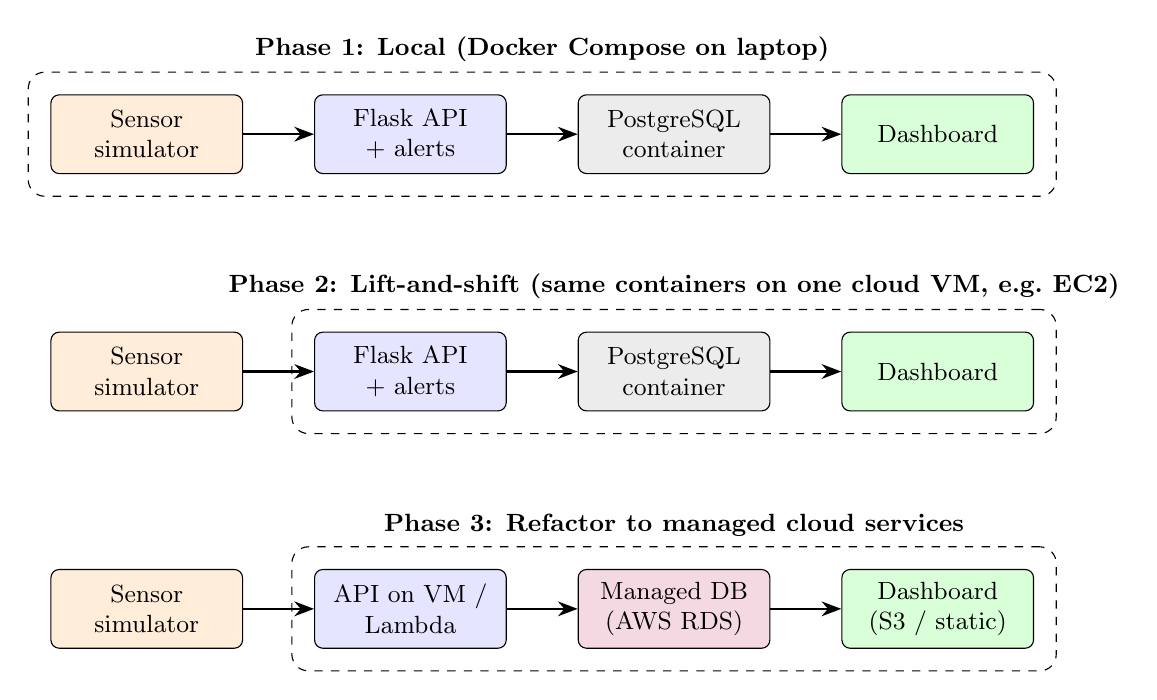
\begin{tikzpicture}[node distance=0.5cm and 0.9cm, every node/.style={font=\small}]
  % Phase 1
  \node[box=orange!15, text width=2.2cm] (s1) {Sensor\\simulator};
  \node[box=blue!10, right=of s1, text width=2.2cm] (api1) {Flask API\\+ alerts};
  \node[box=gray!15, right=of api1, text width=2.2cm] (db1) {PostgreSQL\\container};
  \node[box=green!15, right=of db1, text width=2.2cm] (ui1) {Dashboard};
  \draw[arr] (s1) -- (api1); \draw[arr] (api1) -- (db1); \draw[arr] (db1) -- (ui1);
  \begin{scope}[on background layer]
  \node[layer, fit=(s1)(ui1), label={[font=\small\bfseries]above:Phase 1: Local (Docker Compose on laptop)}] {};
  \end{scope}
  % Phase 2
  \node[box=orange!15, text width=2.2cm, below=2.0cm of s1] (s2) {Sensor\\simulator};
  \node[box=blue!10, right=of s2, text width=2.2cm] (api2) {Flask API\\+ alerts};
  \node[box=gray!15, right=of api2, text width=2.2cm] (db2) {PostgreSQL\\container};
  \node[box=green!15, right=of db2, text width=2.2cm] (ui2) {Dashboard};
  \draw[arr] (s2) -- (api2); \draw[arr] (api2) -- (db2); \draw[arr] (db2) -- (ui2);
  \begin{scope}[on background layer]
  \node[layer, fit=(api2)(ui2), label={[font=\small\bfseries]above:Phase 2: Lift-and-shift (same containers on one cloud VM, e.g.\ EC2)}] {};
  \end{scope}
  % Phase 3
  \node[box=orange!15, text width=2.2cm, below=2.0cm of s2] (s3) {Sensor\\simulator};
  \node[box=blue!10, right=of s3, text width=2.2cm] (api3) {API on VM /\\Lambda};
  \node[box=purple!15, right=of api3, text width=2.2cm] (db3) {Managed DB\\(AWS RDS)};
  \node[box=green!15, right=of db3, text width=2.2cm] (ui3) {Dashboard\\(S3 / static)};
  \draw[arr] (s3) -- (api3); \draw[arr] (api3) -- (db3); \draw[arr] (db3) -- (ui3);
  \begin{scope}[on background layer]
  \node[layer, fit=(api3)(ui3), label={[font=\small\bfseries]above:Phase 3: Refactor to managed cloud services}] {};
  \end{scope}
\end{tikzpicture}
\caption{The three migration phases of our Mini-Predix exercise.}
\end{figure}

\subsection{Migration phases}
\begin{enumerate}
  \item \textbf{Phase 1: Local.} All components run as Docker containers on a laptop using Docker Compose. This is our
        ``on-premises'' baseline.
  \item \textbf{Phase 2: Lift-and-shift (rehost).} The same Docker Compose setup is deployed unchanged on a single
        cloud VM, such as AWS EC2 (free tier). The dashboard gets a public URL.
  \item \textbf{Phase 3: Refactor / replatform.} The PostgreSQL container is replaced with a managed database
        (AWS RDS). Optionally, the ingestion API is moved to a serverless function (AWS Lambda + API Gateway) or the
        sensor feed to AWS IoT Core, and the dashboard is hosted as a static site on S3.
\end{enumerate}

\subsection{Technology stack}
\begin{center}
\begin{tabularx}{\linewidth}{@{}p{3.6cm}L@{}}
\toprule
\textbf{Part} & \textbf{Technology} \\
\midrule
Language & Python 3 (Flask or FastAPI), HTML/JavaScript with Chart.js \\
Containers & Docker, Docker Compose \\
Cloud & AWS (EC2, RDS, optionally Lambda, API Gateway, IoT Core, S3) \\
Load testing & Locust or k6 \\
Monitoring & AWS CloudWatch, application logs \\
Cost estimation & AWS Pricing Calculator, AWS Billing dashboard \\
Version control & GitHub with weekly commits \\
\bottomrule
\end{tabularx}
\end{center}

\subsection{Experiments and measurements}
\begin{center}
\begin{tabularx}{\linewidth}{@{}p{3.6cm}L@{}}
\toprule
\textbf{Metric} & \textbf{How we will measure it} \\
\midrule
Migration effort & Hours spent and number of code/config changes for each phase \\
Latency & Average and 95th-percentile API response time under load (Locust) \\
Throughput & Maximum readings per second before errors increase \\
Cost & Monthly cost of each phase using the AWS Pricing Calculator and billing data \\
Reliability & What happens when the server or database restarts; recovery time and data loss \\
Operational work & Tasks we must do ourselves (backups, patching, scaling) vs.\ handled by the provider \\
\bottomrule
\end{tabularx}
\end{center}
The results will be shown as tables and graphs (for example, latency vs.\ number of simulated sensors for each phase)
and compared with the lessons from the GE case.

\subsection{Expected outcome}
We expect Phase 2 to be quick to set up but to give few cloud benefits, just like a pure lift-and-shift. Phase 3
should need more initial effort but reduce operational work (automatic backups, patching and easier scaling), at a
somewhat higher monthly cost for the managed database. This trade-off is the same one GE faced at much larger scale.

\subsection{Schedule}
\begin{center}
\begin{tabularx}{\linewidth}{@{}p{2.4cm}L@{}}
\toprule
\textbf{Week} & \textbf{Work} \\
\midrule
Week 2 & Detailed report, final design, GitHub repository setup, Phase 1 started \\
Week 3 & Finish Phases 1--3, deploy live, run load tests, collect cost and latency data \\
Week 4 & Analyse results, add graphs to the report, final submission \\
Week 5 & Viva and live demonstration \\
\bottomrule
\end{tabularx}
\end{center}

%================ 8 ROLES ================
\section{Team Roles}
\begin{center}
\begin{tabularx}{\linewidth}{@{}>{\raggedright\arraybackslash}p{3.2cm}>{\raggedright\arraybackslash}p{3.6cm}L@{}}
\toprule
\textbf{Member} & \textbf{Role} & \textbf{Responsibilities} \\
\midrule
Nidhi Dodiya (202303009) & Application developer & Sensor simulator, Flask API, alert logic, dashboard, Docker Compose setup \\
Param Savjani (202303046) & Cloud and testing lead & VPS and AWS setup (EC2, RDS), Phases 2 and 3 deployment, load testing, cost measurement \\
Vraj Makwana (202301436) & Research and documentation lead & Case study research, report writing, architecture diagrams, final report editing \\
\bottomrule
\end{tabularx}
\end{center}
All members will contribute to the GitHub repository, review each other's work, and prepare for the viva together.
Progress is tracked through regular commits and the project documents.

%================ 9 CONCLUSION ================
\section{Conclusion}
The GE Predix case shows both the promise and the difficulty of cloud transformation in a traditional industrial
company. GE correctly identified that industrial data, edge computing and digital twins could create great value,
and its internal migration to AWS reduced the burden of running data centers. However, trying to build and sell a
general-purpose industrial cloud proved too costly and too broad. The main lesson is to rely on public cloud
infrastructure and managed services, and to focus engineering effort on the specific problem being solved.

Our Mini-Predix exercise will reproduce this journey on a small scale, from a local Docker setup, to a cloud VM, to
managed services, and will measure the real differences in effort, cost, performance and reliability.

%================ REFERENCES ================
\section*{References}
\addcontentsline{toc}{section}{References}
\begin{enumerate}[label={[\arabic*]},leftmargin=2.2em,itemsep=5pt]
  \item GE Press Release, ``GE Announces Predix Cloud'', Aug 2015. \url{https://www.ge.com/news/press-releases/ge-announces-predix-cloud-worlds-first-cloud-service-built-industrial-data-and}
  \item Cloud Foundry Foundation, ``A Platform for the Internet of Very Important Things''. \url{https://www.cloudfoundry.org/blog/a-platform-for-the-internet-of-very-important-things/}
  \item Data Center Knowledge, ``GE Unveils Predix, Its Industrial Strength Cloud'', 2015. \url{https://www.datacenterknowledge.com/cloud/ge-unveils-predix-its-industrial-strength-cloud}
  \item Constellation Research, ``GE, Capital One Give AWS the Rub at re:Invent'', 2015. \url{https://www.constellationr.com/content/ge-capital-one-give-aws-rub-reinvent}
  \item Amazon Press, ``General Electric Names AWS Its Preferred Cloud Provider'', Oct 2017. \url{https://press.aboutamazon.com/2017/10/general-electric-names-aws-its-preferred-cloud-provider}
  \item GE Digital, ``Predix Platform for the Industrial Internet'' Datasheet. \url{https://www.ge.com/digital/sites/default/files/download_assets/Predix-Platform-for-the-Industrial-Internet-Datasheet.pdf}
  \item CIO Dive, ``Have GE's Digital Transformation Efforts Hit a Snag?'', 2017. \url{https://www.ciodive.com/news/have-ges-digital-transformation-efforts-hit-a-snag/503736/}
  \item CIO Dive, ``GE to Scale Back Predix amid Companywide Restructure'', 2017. \url{https://www.ciodive.com/news/ge-to-scale-back-predix-amid-companywide-restructure/510758/}
  \item POWER Magazine, ``GE Shelves Plans to Spin Off Digital Business'', 2019. \url{https://www.powermag.com/ge-shelves-plans-to-spin-off-digital-business/}
\end{enumerate}

\end{document}
